



\begin{example2}{Beispiel DEA (eindeutig)} Sprache: $L(M)=\left\{1 x 1 \mid x \in\{0\}^{*}\right\}$
    
    \begin{minipage}{0.45\linewidth}
        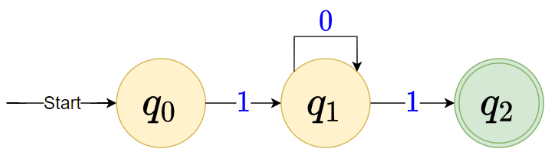
\includegraphics[width=1\linewidth]{images/dea_example.png}
    \end{minipage}
    \hspace{1mm}
    \begin{minipage}{0.5\linewidth}
        \textbf{Konfiguration} auf $\omega=101$
        \begin{itemize}
        \item Startkonfiguration $\rightarrow\left(q_{0}, 101\right)$
        \item Endkonfiguration $\rightarrow\left(q_{2}, \varepsilon\right)$
        \end{itemize}
    \end{minipage}

    \textbf{Berechnung}

    \resizebox{\linewidth}{!}{
    $\omega=101 \rightarrow\left(q_{0}, 101\right) \vdash_{M}\left(q_{1}, 01\right) \vdash_{M}\left(q_{1}, 1\right) \vdash_{M}\left(q_{2}, \varepsilon\right) \rightarrow \text{akzeptierend}$\\
    }

    \resizebox{\linewidth}{!}{
    $\omega=10 \rightarrow\left(q_{0}, 10\right) \vdash_{M}\left(q_{1}, 0\right) \vdash_{M}\left(q_{1}, \varepsilon\right) \rightarrow \text{verwerfend}$
    }
\end{example2}

\begin{example2}{NEA (nicht eindeutig)} Sprache: $L(M)=\left\{x 01 \mid x \in\{0,1\}^{*}\right\}$
    
    \begin{minipage}{0.55\linewidth}
        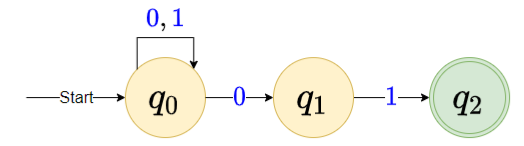
\includegraphics[width=1\linewidth]{images/nea_example1.png}
    \end{minipage}
    \hspace{1mm}
    \begin{minipage}{0.4\linewidth}
        \includegraphics[width=1\linewidth]{images/äquivalenter_nea.png}
        
        äquivalenter DEA
    \end{minipage}    
\end{example2}

\begin{remark}
    KA auf englisch: PDA = Push Down Automat
\end{remark}

\begin{KR}{Kellerautomat für kontextfreie Sprache} $\left\{0^{n} 1^{n} \mid n>0\right\}$
    \begin{itemize}
    \item $0,0 / 00 \quad$ Read $0 \quad$ Add $0 \quad(00-0)=0$
    \item $0, \$ / 0 \$ \quad$ Read 0 Add $0 \quad(\$ 0-\$)=0$
    \item $1,0 / \varepsilon$ Read 1 Remove 0 Read $(\varepsilon-0)=-0$
    \item $\varepsilon, \$ / \$ \quad$ Read $\varepsilon$ - $(\$-\$)=\varepsilon$
    \end{itemize}

    \begin{minipage}{0.5\linewidth}
        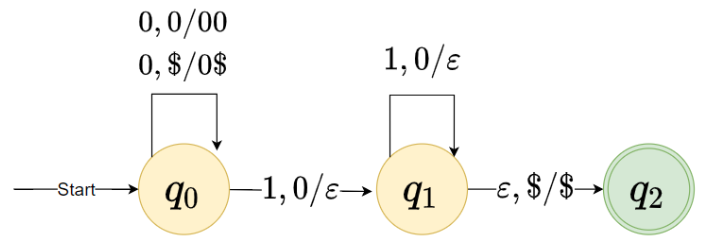
\includegraphics[width=1\linewidth]{kellerautomat_sprache.png}
    \end{minipage}
    \begin{minipage}{0.5\linewidth}
        $\omega_{1}=011:$

        \resizebox{\linewidth}{!}{
        $(q_{0}, 011, \$) \vdash(q_{1}, 11,0 \$) \vdash(q_{1}, 1, \$)$}
        $\rightarrow \omega_{1}$ verwerfend 
        
        Das Zeichen \$ zeigt an, dass der «Stack» leer ist.
    \end{minipage}
\end{KR}

\begin{concept}{NKA}Nichtdeterministischer KA für $\left\{\omega \omega^{R} \mid \omega \in\{0,1\}^{*}\right\}$\\
    
    \includegraphics[width=0.5\linewidth]{nka_übergangsfunktion.png}
\end{concept}

\begin{concept}{Arten von TMs} $\forall$ Sprachen L gleich akzeptierend wie normale TM

    \vspace{1mm}

    \begin{minipage}{0.45\linewidth}
        \begin{itemize}
            \item semi-unendliches Band
            \item mit Speicher
            \item mit Zählern
        \end{itemize}
    \end{minipage}
    \begin{minipage}{0.45\linewidth}
        \begin{itemize}
            \item mehrere Stacks
            \item mehrere Spuren
            \item mehrere Bändern
        \end{itemize}
    \end{minipage}
\end{concept}



\begin{example2}{Mehrband-Maschine}\\
    Spezifizieren Sie eine TM $M_{4}$, welche die Subtraktion von zwei natürlichen Zahlen $(a-b$, mit $a \geq b)$ realisiert.\\
    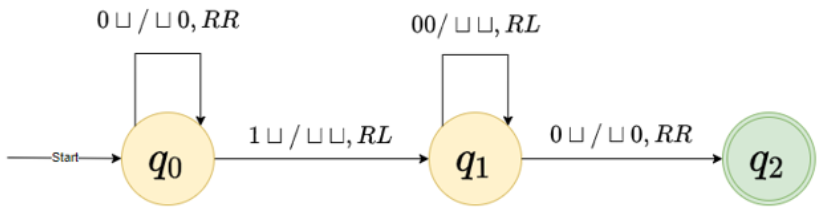
\includegraphics[width=0.5\linewidth]{mehrband_maschine1.png}\\
    Beispiel: $4-2=2$\\
    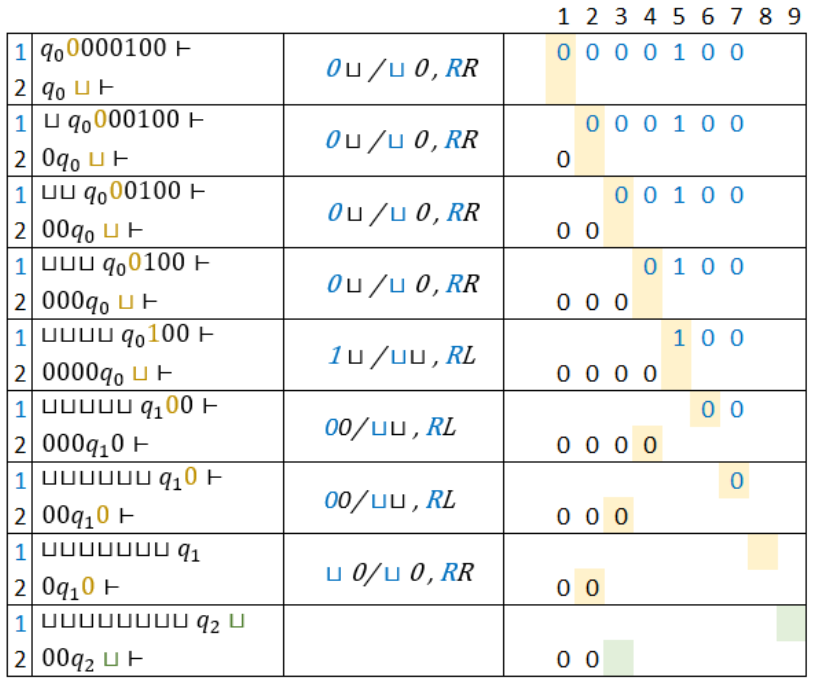
\includegraphics[width=1\linewidth]{mehrband_maschine2.png}
\end{example2}

\begin{example} 
Zeige: Jeder EA für die Sprache $L(M_9)=\{w \in\{0,1\}^{*} \mid| w|_{0} \bmod 3=1\}$ hat mindestens 3 Zustände.\\
1. Jeder EA für $L\left(M_9\right)$ muss die Anzahl der gelesenen Nullen modulo 3 zählen und unterscheiden können.\\
2. Zum Beispiel: $x_1=\varepsilon, x_2=0, x_3=00$\\
3. Widerspruch für alle Paare von Wörtern aufzeigen:\\
Für $x_1$ und $x_2: \quad z_{12}=\varepsilon \quad \Rightarrow \quad x_1 z_{12}=\varepsilon \notin L, \quad x_2 z_{12}=0 \in L$\\
Für $x_1$ und $x_3: \quad z_{13}=0 \quad \Rightarrow \quad x_1 z_{13}=0 \in L, \quad x_3 z_{13}=000 \notin L$\\
Für $x_2$ und $x_3: \quad z_{23}=\varepsilon \quad \Rightarrow \quad x_2 z_{23}=0 \in L, \quad x_3 z_{23}=00 \notin L$\\
4. Jeder EA für $L\left(M_9\right)$ muss zwischen mindestens drei Zuständen unterscheiden. Der EA hat mind. 3 Zustände.
\end{example}

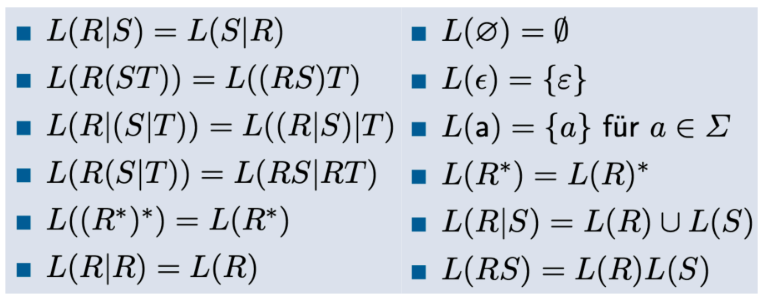
\includegraphics[width=1\linewidth]{regeln_dings.png}